\chapter[2024 March]{March 2024}

\section{March Schedule}

\TabRef{tab:schedule_03} Shows the EPR 402 schedule for March 2024.
\begin{table}[H]
  \centering
  \caption{EPR 402 Schedule for March 2024}
  \label{tab:schedule_03}
    \begin{tabular}{ !{\vrule width 1.1pt}
                    c!{\vrule width 1pt}
                    c!{\vrule width 1pt}
                    c!{\vrule width 1pt}
                    p{8.6cm}!{\vrule width 1pt}}
    \noalign{\hrule height 1pt}
    \cellcolor[gray]{0.9} \textbf{Week} &
    \cellcolor[gray]{0.9} \textbf{Date} &
    \cellcolor[gray]{0.9} \textbf{Part} &
    \cellcolor[gray]{0.9} \textbf{Required reading / Assignment due date }
    \\ \noalign{\hrule height 1pt}
    1     &   4 Mar --   8 Mar & 1 & Literature study and reading.
    \\ \hline
    2     &   11 Mar --   15 Mar & 1 & Literature study and reading
    \\ \hline
    3     &  18 Mar --  20 Mar & 1 & Project proposal draft
    \\ \hline
       &  20 Mar --  31 Mar &   & Recess
    \\ \hline
    \end{tabular}
\end{table}

\pendsign

\section[2024/03/01]{Friday, 1 March 2024}
\label{sec:01_march}

\subsection{Project: Intelligent Web Application Firewall using JSON Web Token Inspection}

Next-generation firewalls, also called Web Application Firewalls (WAFs), have significantly improved the defence capabilities of organisations against common web application attacks. These devices perform deep-packet inspection of traffic to detect and alert on anomalies in the HTTP requests and responses. Although these devices can detect common attacks such as cross-site scripting and SQL injection, they still lack the intelligence required to detect attacks masquerading as normal behaviour such as business logic flaws or authorisation bypasses.

However, with the latest move towards decentralised authentication mechanisms, such as JSON Web Tokens (JWTs), which contain information such as user claims, it may be possible to incorporate this information to detect more complex attacks.

The project student is expected to deliver a standalone device that can leverage existing detection techniques and new information that can be found in the claims of tokens to detect more complex attacks such as authorisation bypasses. Using machine learning techniques that incorporate this new information, the student should develop a system that can better learn normal behaviour to detect and alert on complex anomalies.

\textbf{Nature of the work}
\begin{itemize}
    \item A standalone device that can act as a WAF and detect more complex attacker techniques such as authorisation bypasses will be implemented.
\end{itemize}

\subsection{Research Ideas}
\begin{compactitem}
\item Web Application Firewalls
\item Heuristic-based anomaly detection
\item Token-based access control
\item Read and summarise: Next Generation Firewall for Network Security: A Survey \cite{8478973}
\item Read and summarise: Critical Analysis on Web Application Firewall Solutions \cite{6513431} 
\end{compactitem}

\todoredefined{Should do a search to identify any relevant papers and articles }

\subsection{Literature Review}
\subsubsection{Next Generation Firewall for Network Security: A Survey \cite{8478973}}
    The authors of this paper attempt to understand what differentiates next-generation firewalls (WAF's) from traditional firewalls we are generally used to. They go into depth to see which features these firewalls use that make them desirable and what traditional firewalls lack in the modern age. These authors list commonly occurring cyber attacks and how each firewall deals with each attack. The authors also compare the advantages and disadvantages of each firewall.
    
    The performance benchmarks used by the authors are Advanced Evasion Techniques, Targeted Cyber-Attack, Web Application Attacks, and Data Focused Attacks. The authors also compare the differences between the two firewalls in the following areas: Preventing Advanced Persistent Attacks, Inspecting SSL Traffic, Controlling Web Applications, Managing Users \& Use Policy and Trade off Security vs Performance.
    
    Overall this paper does not go into too much technical detail about what WAF's do and how they operate, but the authors make the point that it is necessary because of its advantages over traditional firewalls. Finally, the authors look at an example of the Palo Alto Next-Generation Firewall and how it manages to extend its functionality over traditional firewalls.

\subsubsection{Critical Analysis on Web Application Firewall Solutions \cite{6513431}}
    This paper compares existing WAF solutions to see which gaps exist in which solutions. The authors make the argument that certain solutions have certain features that make them a better fit for certain scenarios. Solutions that are being compared include Mod Security, Imperva's Secure Sphere, Barracuda network application gateway etc. 

    The paper goes into some technical detail on how and where WAF's operate. WAF's work on OSI layer 7, the application layer by deeply inspecting the HTTP packet and directing and analyzing it for malicious strings and configuration error problems. The authors compare all the options using metrics like Time efficiency, how well its organised, Effectiveness, if it has Monitoring, Blinking, Response Filtering, Attack Prevention, Web Site Cloaking, Authentication and Web SSO, Deep Inspection, Session Protection and finally evaluate the Overall Security Performance.

    The researchers also compare the management interface of the WAF applications using the following metrics: Web Based, Command Line, Desktop Based, Ease-of-use, Comprehensiveness and Flexibility. The authors make a final observation that WAF's have become essential for each website and can become highly customized, but depending on your business needs a best fit solution can be found.

\subsubsection{Fast Pattern Matching in Compressed Data Packages \cite{5700208}}
The authors of this paper explore Fast Pattern Matching which can significantly speed up Firewalls and intrusion prevention systems by leveraging deep packet inspection of compressed data packages in high-speed systems. The authors attempt to leverage hardware Huffman encoding by only decompressing data once and then filtering similar packets since the system does not need to decompress packets with the same source and destination address as the first decompressed packet.

The authors explain that this is also an important step in ad filtering since keyword searches for ad-related words in the decompressed packages can also be searched for. According to the authors, this method has enormous speed increases compared to pure software encoding.

\subsubsection{A Fully Automated Deep Packet Inspection Verification System with Machine Learning \cite{7947802}}
The authors of this paper created a deep packet inspection (DPI) verification system for growing network density and Quality of Service. The authors use mobile automation tools like Monkey Runner, UI Automator, Monkey Talk, Appium and GUITAR to simulate application web traffic. This is easier than generating application web traffic using a mobile web browser since not a lot of tools for this exist.

The authors explore doing Automated Application Signature Verification for the HTTP Packets. The solution works by running a command-line packet sniffer and network protocol analyzer to see all the HTTP traffic. From this an include/exclude list which contains specific keywords that are either blocked or allowed. The packets are inspected and allowed or blocked based on the specific keyword. This is done differently for HTTP, SSL, TCP and UDP.

The proposed script generates a list of relevant flows based on the SSL, TCP or UDP flow size and rate. The verification system detects the flow rates and flags any suspicious flow rates. The final result is a fully automated signature verification system of the flow rates.

\subsubsection{Core Problems}
\textbf{Primary Problems}
\begin{enumerate}
    \item \textbf{JWT Inspection:}\\
        The product needs to parse incoming JWT tokens to extract claims and verify their integrity and authenticity, validate JWT signatures to ensure they haven't been tampered with and check the expiration time, issuer, and audience of the JWT token to prevent token replay attacks. It also needs to monitor JWT usage patterns to detect abnormal JWT behaviour, such as excessive token creation or usage from unexpected locations.
    
    \item \textbf{Heuristic-Based Anomaly Detection:}\\
        The product needs heuristics to identify abnormal patterns in incoming HTTP requests which may include request rate, payload size, header analysis, HTTP method, user agent analysis, etc. It also needs to implement algorithms to detect anomalies based on these heuristics. Machine learning algorithms such as clustering, decision trees, or neural networks can be used for anomaly detection.

    \item \textbf{Integration with Web Application Firewall:}\\
        The product needs ensure the WAF can intercept incoming HTTP requests before they reach the application server and implement rules to block or allow requests based on the results of anomaly detection and JWT inspection.
\end{enumerate}

\textbf{Secondary Problems}
\begin{enumerate}
    \item \textbf{Continuous Monitoring and Updates:}
        Continuously monitor the performance of the WAF and adjust heuristics and detection algorithms as needed.

    \item \textbf{Logging and Reporting:}
        Log all WAF actions, including blocked requests, allowed requests, and detected anomalies.

    \item \textbf{Testing and Deployment:}
        Thoroughly test the WAF in a staging environment, monitoring its performance and effectiveness in real-world scenarios.

    \item \textbf{Documentation and Training:}
        Document the WAF's configuration, rules, and operational procedures to train administrators and developers on how to use and configure the WAF effectively.

\end{enumerate}

\pendsign

\section[2024/03/04]{Monday, 4 March 2024}

\subsection{Research Ideas}

\begin{compactitem}
\item Research some more papers with a more technical approach to WAFs.
\item Find out more about JWTs on Google.
\item Find out which features and functions a WAF has.
\end{compactitem}

\todoredefined{Should do a search to identify and summarise any relevant technical papers}

\subsection{Literature Review}
\subsubsection{A survey of network anomaly detection techniques \cite{AHMED201619}}
This paper proposes an in-depth analysis of classification, statistics, information theory and clustering in anomaly detection techniques. The authors describe the generic framework for network anomaly detection and how it is utilized in most solutions. They also indicate that security incidents had exponential growth in 2009-2014 and anomaly detection has become more important.

The authors describe types of anomalies like point anomalies, contextual anomalies and collective anomalies, how these different anomalies can be detected and the output of different anomaly detection techniques. The authors have a heuristic score where if the anomaly score is above a certain threshold it gets flagged. The types of network attacks like Denial of Service (DoS), Probe, User to Root (U2R) and Remote to User (R2U) are described and how these attacks can be measured by heuristics and how sophisticated the attacks can get.

The paper then follows by describing classification-based techniques, statistical anomaly detection techniques, Information theory and cluster-based techniques and their respective complexities. In conclusion, depending on the attack preference, different techniques can be used to detect the anomalies.

\subsubsection{Deep learning methods in network intrusion detection: A survey and an objective comparison \cite{GAMAGE2020102767}}
This paper investigates the efficiency of different deep learning models on different internet traffic datasets. The paper lists supervised instance learning, supervised sequence learning, semi-supervised instance learning and other learning paradigms as deep learning models. The Internet traffic datasets are of different sizes and are real-world data from web servers with the datasets varying in size from 100 000 instances to 16 million instances.

The weighted macro average of the metrics is taken as the heuristic of the neural network and the results are based on the accuracy of the neural network. The authors explain how they do pre-processing on the data and hyper-parameter configuration. The authors list using legacy datasets as one of the several weaknesses, as well as inadequate details of models leading to inaccurate results that cannot be reproduced.

The results show that deep feed-forward neural networks perform the best overall datasets and are perfect for WAF's that have a large number of packets incoming since the ANN gets more efficient on more data. Since this is application-specific, the ANN does not do well on small web servers.

\pendsign

\section[2024/03/05]{Tuesday, 5 March 2024}

\subsection{JWTs}

JWTs have the following structure according to \cite{JWTIO}:

\begin{figure}[H]
    \centering
    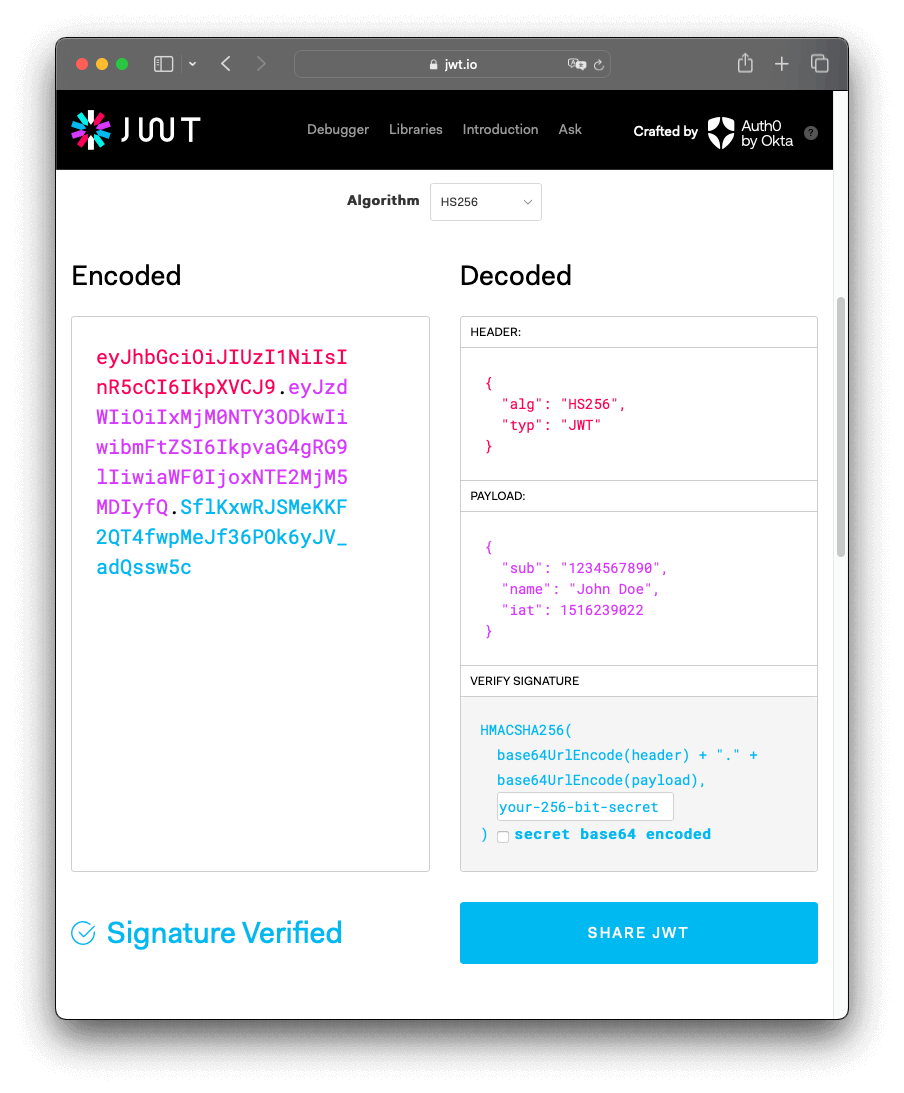
\includegraphics[width=0.5\textwidth]{2024/Images/Theoretical Background/debugger.png}
    \caption{JWT Structure}
    \label{fig:jwt_structure}
\end{figure}

The JWT contains three elements, namely the header, payload and signature. These are individually base64 encoded in a xxx.yyy.zzz format as can be seen above.

\subsubsection{JWT Header}

The JWT header contains the following information.

\begin{lstlisting}
{
  "alg": "HS256",
  "typ": "JWT"
}   
\end{lstlisting}

The header consists of two parts. The first part is the type of the token, which is JWT in this case, and the second part is the signing algorithm used, such as HMAC SHA256 or RSA.

\subsubsection{JWT Payload}

The JWT payload contains the following information:

\begin{lstlisting}
{
  "sub": "1234567890",
  "name": "John Doe",
  "admin": true
}
\end{lstlisting}

The payload contains the claims of the JWT. Claims are statements about the user and some additional data. Claims fall into one of three categories, namely registered-, public- and private claims.

\begin{itemize}
    \item \textbf{Registered claims} are a set of predefined claims that are not mandatory but recommended. It provides a set of useful and interoperable claims such as \textbf{iss}(issuer), \textbf{exp}(expiration time), \textbf{sub}(subject), \textbf{aud}(audience) among others.
    \item \textbf{Public claims} are claims that can be identified at will by the user of the JWT. They are defined in the JWT registry to avoid collisions in the namespace.
    \item \textbf{Private claims} are custom claims created to share information between parties that agree on them and are not registered or public claims.
\end{itemize}

\textbf{These claims can be used to extract useful information about the user that is not available in normal HTTP requests.} Since the claim contains information about the user, a portfolio about the user can be built up to predict what a user will or will not do and if a user acts outside of this framework, it can be logged as an anomaly.

\subsubsection{JWT Signature}
The signature, as shown below, is a combination of the encoded header, the encoded payload and a secret which is signed with the algorithm specified in the header.

\begin{lstlisting}
HMACSHA256(
  base64UrlEncode(header) + "." +
  base64UrlEncode(payload),
  secret)
\end{lstlisting}

The signature verifies that the message was not changed along the way between the client and server. If the token is signed with a private key, it also verifies that the sender of the token is the client and not a third party.

\pendsign

\section[2024/03/08]{Friday, 8 March 2024}

\subsection{Research Ideas}

\begin{compactitem}
    \item Do more practical work, try to hack JWTs.
    \item Try and get a DVWA (Damn Vulnerable Web Application) going on a VM.
\end{compactitem}

\todoredefined{Should try and hack a JWT using TryHackMe}

\subsection{WAF Basics}
\textbf{WAFs block the following attacks} according to \cite{WAFATTACKS}
\begin{itemize}
    \item DDOS
    \item SQL Injection
    \item Cross-Site Scripting (XSS)
    \item Zero-day
    \item Business Logic (Circumstantial vulnerabilities)
    \item Man-in-the-middle
    \item Malware
    \item Defacements
\end{itemize}

\subsection{JWT authentication bypass}
According to \cite{JAB2022}, JWT authentication bypasses occur when user claims are modified to gain unauthorised access.

\textbf{JWT authentication bypasses can be prevented by:}
\begin{itemize}
    \item Using modern, up-to-date JWT libraries.
    \item Perform robust signature verification on JWTs and account for edge cases such as using unexpected signing algorithms.
    \item Enforce a strict whitelist of permitted hosts for the \textbf{jku}(JWK Set URL) header.
    \item Ensure the website is not vulnerable to path traversal or SQL injection via the \textbf{kid}(Key ID) header parameter.
\end{itemize}

\pendsign

\section[2024/03/11]{Monday, 11 March 2024}

\subsection{TryHackMe}
Using the tutorial provided by \cite{TRYHACKME}, I tried to hack a JWT. It worked for all the tasks. I learned that it would be difficult to use conventional defence methods to stop JWT authentication bypasses since they are legitimate requests that exploit flaws in web applications.

\subsection{DVWA}
Next, I tried to get the DVWA going on an Ubuntu VM as provided by \cite{DVWA} in order to try and hack the web application on my local network.

I learned that more work will be necessary in this regard since the local network blocks some attacks before they can even reach the host machine.

\pendsign

\section[2024/03/12]{Tuesday, 12 March 2024}

\subsection{Research Ideas}

\begin{compactitem}
    \item Start looking at the Project Proposal.
    \item Try and write the introduction.
    \item Look at the OWASP Top 10.
    \item Look at the OWASP testing suite.
    \item Look at open-source WAF implementations.
\end{compactitem}

\todoredefined{Work on Project Proposal}

\pendsign

\section[2024/03/18]{Monday, 18 March 2024}

\subsubsection{OWASP Top 10 Vulnerabilities}

The OWASP Top 10 are the 10 most common vulnerabilities in web applications at the current time. In 2021, which is the most up-to-date version \cite{OWASPTOP10}, it was indicated as follows:

\begin{enumerate}
    \item Broken Access Control
    \item Cryptographic Failures
    \item Injection
    \item Insecure Design
    \item Security Misconfiguration
    \item Vulnerable and Outdated Components
    \item Identification and Authentication Failures
    \item Software and Data Integrity Failures
    \item Security Logging and Monitoring Failures
    \item Server-Side Request Forgery
\end{enumerate}

\textbf{JWT authentication bypasses} are part of the \textbf{Identification and authentication failures}

\subsubsection{Embedded Device}

Some possible embedded devices include the O-droids. This includes the M1, which is commonly used or the M1S which is a version with the same processor but different GPU cores.

\pendsign

\section[2024/03/20]{Wednesday, 20 March 2024}

\subsection{Research Ideas}

\begin{compactitem}
    \item Look at more vulnerabilities outside of the OWAPS Top 10.
    \item Focus research on WAF accuracy thresholds
    \item Look into one WAF serving multiple web applications.
    \item Keep in mind that both client and server-side attacks need to be included.
    \item Focus on WAF components
\end{compactitem}

\todoredefined{Do more TryHackMe tutorials}
\todoredefined{Complete Project Proposal}
\todoredefined{Focus on functional blocks of a WAF}
\todoredefined{Focus on accuracy of WAF, split into conventional and non-conventional attacks}

\subsubsection{OWASP Testing Suite}
The OWASP Testing Suite is a web application penetration tool to scout for vulnerabilities in web applications, as indicated in \cite{OWASPTESTSUITE}. It could be useful to test against existing web applications and WAFs.

\subsubsection{Open-source WAFs}

Some open-source WAFs according to \cite{OSWAFS}, include:
\begin{itemize}
    \item NAXSI
    \item WebKnight
    \item Shadow Daemon
    \item Coraza
    \item OctopusWAF
    \item IronBee
    \item ModSecurity
\end{itemize}

\pendsign

% \begin{mdframed}[style=redact,
%     frametitle={\textcolor{white}{Redacted,
%         see page~\pageref{sec:20240401} for correct version.}}]

% \subsection{Testing block redaction}

% Testing redaction of entries that contain errors or are no longer relevant.

% \end{mdframed}

% \subsection{Testing local redaction}

% As an alternative, if just a local change must be made to a sentence, the
% follow example shows how this should be done: \st{Example of a redacted
% sentence}\textcolor{ScarletRed}{Replacement text}.

% \pendsign
